\documentclass[conference]{IEEEtran}
\IEEEoverridecommandlockouts
% The preceding line is only needed to identify funding in the first footnote. If that is unneeded, please comment it out.
\usepackage{cite}

\usepackage{amsmath,amssymb,amsfonts}
\usepackage{algorithm}
\usepackage{algorithmic}
\usepackage{graphicx}
\usepackage{textcomp}
\usepackage{xcolor}
\usepackage{listings}

\definecolor{lightgray}{rgb}{.9,.9,.9}
\definecolor{darkgray}{rgb}{.4,.4,.4}
\definecolor{purple}{rgb}{0.65, 0.12, 0.82}
\def\BibTeX{{\rm B\kern-.05em{\sc i\kern-.025em b}\kern-.08em
    T\kern-.1667em\lower.7ex\hbox{E}\kern-.125emX}}
%%========================DEFINING JAVASCRIPT IDENTIFIERS=============
\lstdefinelanguage{JavaScript}{
  keywords={typeof, new, true, false, catch, function, return, null, catch, switch, var, if, in, while, do, else, case, break, list, let, Step},
  keywordstyle=\color{blue}\bfseries,
  ndkeywords={class, export, boolean, throw, implements, import, this, Loop},
  ndkeywordstyle=\color{blue}\bfseries,
  identifierstyle=\color{black},
  sensitive=false,
  comment=[l]{//},
  morecomment=[s]{/*}{*/},
  commentstyle=\color{purple}\ttfamily,
  stringstyle=\color{red}\ttfamily,
  morestring=[b]',
  morestring=[b]
}
\lstset{
   language=JavaScript,
   backgroundcolor=\color{lightgray},
   extendedchars=true,
   basicstyle=\footnotesize\ttfamily,
   showstringspaces=false,
   showspaces=false,
   numbers=left,
   numberstyle=\footnotesize,
   numbersep=2pt,
   tabsize=2,
   breaklines=true,
   showtabs=false,
   captionpos=b
}


\begin{document}

\title{Evolving Behavior using Genetic Algorithm: Natural Selection\\
}

\author{\IEEEauthorblockN{1\textsuperscript{st} Given Name Surname}
\IEEEauthorblockA{\textit{dept. name of organization (of Aff.)} \\
\textit{name of organization (of Aff.)}\\
City, Country \\
email address}
\and
\IEEEauthorblockN{6\textsuperscript{th} Given Name Surname}
\IEEEauthorblockA{\textit{dept. name of organization (of Aff.)} \\
\textit{name of organization (of Aff.)}\\
City, Country \\
email address}
}

\maketitle

\begin{abstract}
The fitness function based method of artificial evolution is asserted to be inadequate for real world entities. Evolutionary computing refers to the paradigm of artificial intelligence without an explicit fitness function. Evolution of entities via natural selection is a way forward.
This paper is an extension of Channon's and Damper's natural selection work and further focus on the principles of development of evolving neural network. To test the extended idea, a world(artificial) containing self evolving organisms is created and described. Rather than writing thoughtful fitness functions, we let a process found in nature-{\textit{evolution}}-decide for us. Results show that such systems are well suited to long-term incremental development system.
\end{abstract}

\begin{IEEEkeywords}
Evolutionary computing, natural selection, neuroevolution
\end{IEEEkeywords}

\section{Introduction}
Evolutionary Computing(EC)\cite{evolvable-machines} is and algorithmic paradigm to solve search and optimization problems using core principles behind Darwinian evolutionary theory. There will be no discussion of protein synthesis, RNA and other topics related to actual biological process, rather we develop algorithms inspired by these principles. Can we think of DNA as  object(brain) to an artificial organism?\cite{Stanley} Can objects generate new objects and pass on their DNA? The answer to the questions is yes. This paper look into biological principles of evolution and find way to apply those in code \cite{algorithms-and-experiments}. We simulate one of the most powerful process found in nature without going into depth of science of genetics. I encourage readers to explore possibilities for expanding the scenario provided and don't care so much on accurate simulation of evolution; rather, care upon applying evolutionary strategies in software.

\section{Technique to evolve behavior}
Artificial life presents us with problem which is difficult to specify to a machine. Therefore we should either increase our grasp on it, or create something which outperform the statements we give it \cite{channon&damper}. The first possibility is not appropriate as it is based on traditional fitness function approach. It also includes manually increasing the understanding and modelling life by impressive systems within their environments.\\
The second option has no explicit evaluation function. Through organism interaction with environment(external stimulus) certain behaviors evolve from them without any long-term goal \cite{soccer-game-evolution}. Algorithm is implemented in specific way to solve organism behavior problem. As evolution is applied to inherently complex problems \cite{algorithms-and-experiments} finding adequate evaluation function becomes an obvious problem. At the same time natural selection is necessary for emergence of new generation of organisms but it doesn't imply sustained emergence. The changes in genotype must be taking place slowly and must be correlated with the fitness evaluation of an organism \cite{mapping-genotype-phenotype}.

\section{What to evolve}
The organisms need to evolve over time so they need a human brain like structure. But how should the brain network be specified? The emergence of new generation requires new neural structures as well. There are various known examples of structures that can serve our purpose.\\
Gene theory is one of the solution. At any stage of development, in any one cell, only a small proportion of genes will be used. The gene lies in the cell and cell in the brain itself. The duplicate system could be obtained either by gene duplication or along with development process.\\
Direct duplication of gene as a source of neural structure duplication is not feasible(as it will only create a copy of parent). Therefore, for constructive evolutionary emergence of complex behavior, a mutation process is required. A newly created organism receive a duplicated copy of its parent, but the development process mutates genes in some constraints; based on some mutation rate. This modular development lead to emergence of new unexpected(may be good or bad) behavior. New combination of features occur and organisms evolve \cite{Stanley}.

\section{Natural Selection Process}
Before we walk into the scenario and algorithm, let's take moment and describe Darwinian principles of evolution that will be required in our simulation. For the simulated natural selection process to occur as it does in nature, three of these elements must be present.
\begin{enumerate}
\item \textbf{Heredity.} It is the process by which parent properties or genes are transferred to children. The traits are passed down to their children in the next generation of organisms, if they live enough to reproduce. Hence the newly created organism's brain will be inherited from parent.
\item \textbf{Variation.} Diversity of traits must be present in the population or a means to introduce variety must exist. Consider the example: A population of organisms in which all are exactly same: same color, same size, same everything. There is no variety in population; the children will always be identical to either parent or to each other. Nothing can evolve as new combination of traits will never happen.
\item \textbf{Selection.} This is the mechanism by which some of the population have the chance to pass down their genetic information and some do not. Such a model is called \textit{survival of the fittest.}
For example: A goat population is chased by lions every day. The faster once are likely to escape from the lions and can live longer and have a chance to reproduce to pass down their genes to their children. The term "fittest" however, can be misleading. It has no relation with organism being physically fit. In the case of our example, we define our own fitness criteria based on the environment.
\end{enumerate}

\section{The Neural System: DNA Encoding}
\subsection{Scenario}
We create an artificial life scenario to validate the above. The Asystem is a world which contain food, poison and organisms. The population of organisms will survive or die eating food or poison. Each creature has attraction and repulsion to food and poison. Along with this, they have an extent to sense food and poison; so they only eat those which are in their scope. The one with greater extent to sense food with higher repulsion to poison lives longer and get chance to reproduce, and the one with lesser attraction to food die early.

\subsection{Genotype}
The digital information-the actual genetic code is an organisms \textbf{genotype}. In simple words, it is the data that simulate the brain functionality. From generation to generation this information is passed down. What are entities in the world? How to design the genotype for the entities? What data structure would you use to store the properties? How to choose the encoding for the system? Attention to be paid to developing system in which children's network must resemble parent aspects-keeping in mind Darwinian principle of heredity.\\
Taking into account the proposed development environment system, each organism's DNA must have the following:
\begin{enumerate}
\item \textbf{Attraction/Repulsion to food}
\item \textbf{Attraction/Repulsion to poison}
\item \textbf{Radius to sense food}
\item \textbf{Radius to sense poison}
\end{enumerate}
The key part is that each member of population has a virtual \textit{DNA}. These above mentioned properties become "genes" for organism. This set out how an organism will look or behave. Based on this DNA an organism will move in the system(left, right, up, down). The sensing proportion of the gene will sense the food in scope and remaining proportion decide whether it should be eaten or not(attraction or repulsion). The DNA drives the behavior of organism.\\
The DNA is encoded as an array of floating point numbers of size equal to the set of properties. It is randomly initialized at the time of construction. Encoded value is a non-zero lying within the constraints. We also define attraction/repulsion range between -3 and 3 and radius range as 5 to 100 pixels.
%%===========================GENOTYPE FIGURE==========================
\begin{figure}
	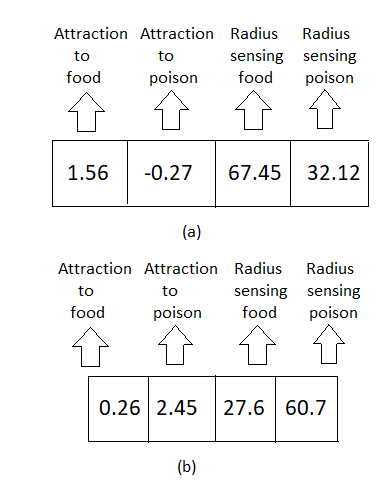
\includegraphics[scale=1]{genotype.png}
	\caption{Genotype: DNA encoding for an organism}
	\label{fig:genotype}
\end{figure}
Figure \ref{fig:genotype} shows DNA of two different organisms. The first one is more attracted to food with higher food sensing scope whereas the second one is much attracted to poison with greater poison sensing radius. Clearly, the later one would not be able to survive for long and get chance to reproduce. This defines the organisms character. The more the organism can sense food with higher attraction or the more the organism is repulsive to poison, the better it is for survival.

\section{Development System}
For simulating natural system, let's look at a way in which we use genetic algorithm to build something that resembles the \textit{ecosystem}. We create organisms(triangular shape) that moves about the screen searching food. Higher the sensing radius, the more it can locate and decide whether to eat or not.

\begin{lstlisting}[caption = DNA of Organism]
class Organism {
	this.dna = [random(-3,3), random(-3,3), random(5,100), random(5,100)];
	this.health;
	.....
}
\end{lstlisting}
We will store the population of organisms in a list(not in array) as we expect population to grow and shrink as how often organisms die or are born. We initialize the elements of list as organisms.
\begin{lstlisting}[caption = Making initial population of organisms]
let world_population = 500;
list<Organism> population;
for (let i = 0; i < world_population; i++) {
	population.add(new Organism());
}
\end{lstlisting}
So far we have an organism that moves across the window and code that manages variable number of organisms. To make it into a system that evolves, we add features to our world:
\begin{itemize}
\item \textbf{Organism die}
\item \textbf{Organisms are born}
\end{itemize}
Organism dying acts as a replacement for fitness function. If organism dies, it no longer exits and cannot be selected to be parent! To ensure deaths in world we add health variable to Organism class(listing 1). An organism gets 100 health points when born. In each iteration of loop(animation) organism loses some health.
\begin{lstlisting}[caption = Updating death variable]
void update() {
	this.health -= 1;
}
\end{lstlisting}
If organism health drops down to 0, it dies.
\begin{lstlisting}[caption = Function in organism class to test if dead or not]
boolean dead() {
	if (health < 0.0) 
		return true;	
	return false;
}
\end{lstlisting}
Perhaps you are thinking that all organisms start with 100 points and loses 1 point per iteration, then all will live for same amount of time and then die together. If this happens then there will be nothing to evolve. Hence we introduce food and poison. Organisms life is extended when it eats food as this increases its health points.\\
let's assume \textit{food}(and \textit{poison}) as list of vector co-ordinates of food(and poison). If food(or poison) lies in proximity, it eats food(or poison) and increase(or decrease) its health.
\begin{lstlisting}[caption = Eating food and poison]
void eatFood() {
	for (let i = food.size() - 1; i >= 0; i--) {
		let food_location = food.get(i);
		let	distance = dist(food_location, this.location);
		if (distance < this.dna[2]) {		// Food sensing gene
			health += 100;
			food.remove(i);
		}
	}
}
void eatPoison() {
	// Same as above. Just subtract health. Use dna[3]
	....
}
\end{lstlisting}
In this scenario organisms can eat food to live longer and have likelihood to reproduce. The system will evolve organisms with ability to find and eat food.

\section{Genotype and Phenotype}
Its important to know distinction between concepts of \textit{genotype} and \textit{phenotype}. The actual genetic data Figure \ref{fig:genotype} is element's genotype. The \textbf{phenotype}, however, is the expression of that data. This decides how we use genetic algorithm in our work \cite{mapping-genotype-phenotype}. How will we outline genotype to visualize it as phenotype? What does genotype variables express? This is done by graphic programming. Consider probably simplest color example in Figure \ref{fig:genotype-and-phenotype}. As you see, genotype is digital data stored in integer variables and we choose to express that integer as color. But choosing expression for data is arbitrary. In other scenarios, you can use these integers to express length of line, weight of force etc. How can we express our organism? What could be the phenotype?\\
The organisms ability to locate food(or poison) is tied to two variables(genes)-
\begin{enumerate}
\item \textbf{Sensing genes.} To what extent organism can locate food(or poison)
\item \textbf{Attraction/Repulsion genes.} How quickly it moves toward the food(or poison)
\end{enumerate}
Organisms with higher sensing power find food more often and one with higher attraction power cover more ground in shorter period of time.
%%===========================GENOTYPE AND PHENOTYPE=================
\begin{figure}
	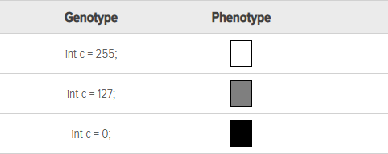
\includegraphics[scale=1]{genotype-and-phenotype.png}
	\caption{Phenotype visualizing corresponding to Genotype}
	\label{fig:genotype-and-phenotype}
\end{figure}
%%===========================PHENOTYPE===========================
\begin{figure}
	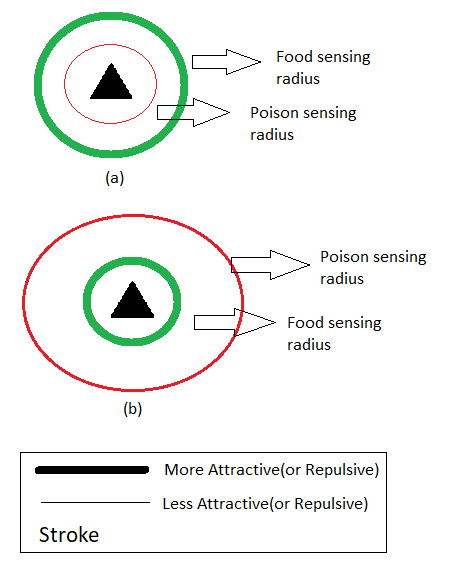
\includegraphics[height=7cm,width=7cm]{phenotype.png}
	\caption{Phenotype: Expression of virtual DNA}
	\label{fig:phenotype}
\end{figure}
\\Figure 3 shows organism is represented in a triangular shape, and DNA phenotype is the circles around it. The two circles tend to locate food and poison and attraction/repulsion power is represented by stroke of circles. The more the stroke the more it tends to move towards the food or poison. Stroke is just mapping of steering force(attractive or repulsive) to circle outline width.
\begin{lstlisting}[caption = Adding Phenotype in Organism class]
void display() {
	// Draw the triangle..
	// Set stroke using a mapping function on dna[0] for food
	// Set stroke using a mapping function on dna[1] for poison
	// Draw food cicle using dna[2]
	// Draw poison circle using dna[3]
}
\end{lstlisting}

\section{Selection and Reproduction}
\subsection{Selection}
Now having genotype and phenotype, we move to next step to devise a means for organisms to be selected as parents. As stated above longer living organisms have more chance to reproduce. The life length of organisms is its \textit{fitness}.\\
One possibility could be to presume that whenever two organisms come in proximity of each other, they make a new organism \cite{improving-neuroevolution}. The longer an organism lives, the more probable it is to come in scope with another organism. So in addition to eating food, they also need to find another organism for the likelihood of having child.\\
Other possibility would be to have \textit{asexual} reproduction. An organism will not require a partner. At any moment, it can make a clone of itself. The cloned organism will have same genetic make-up. So selection algorithm becomes:\\
\textbf{\textit{At any instant, organism has 1\% chance of reproducing.}}\\
The longer an organism lives, the more chance is there that it make atleast one child. Selection algorithm can be implemented by writing function in Organism class that harvest a random number every iteration(animation frame). If picked number is lesser than 0.01(1\%), a new organism is born.
\subsection{Reproduction}
How does an organism reproduce? The reproduction process will involve a function in Organism class that will make a new organism object from newly made DNA. Since single parent is making a child, we call a \textit{copy} function instead. It copies the content of one array into the another.
\begin{lstlisting}[caption=Function returning new organism: the child]
Organism reproduce() {
	if(random(1) < 0.005) {
		let child_dna = copy();  // Make copy of dna	
		mutate(child_dna, 0.01);
		return new Organism(location, child_dna);
	} else return null;
}
\end{lstlisting}
The child is born at same location as that of parent. Also note we've reduced reproduction probability from 1\% to 0.5\%. This makes a huge variation; with greater probability the ALife will rapidly move in direction of overpopulation. A lower probability, and everything will die out quickly. Once child DNA is created we put in the final process before adding it to the next generation-\textit{mutation}. It exist because of principle of variation. It permits to introduce diversity through evolutionary process itself \cite{Stanley}.\\
Mutation is expressed in terms of mutation rate. Genetic algorithm might have 1\% or 0.5\% etc. as mutation rate. A mutation rate of 1\% means that there is 1\% chance that it will mutate the gene. What does it mean to mutate? In this case, mutation means adding some random value to the gene. This random value could be positive or negative depending on the constraint described.\\
%%===========================MUTATION===========================
\begin{figure}
	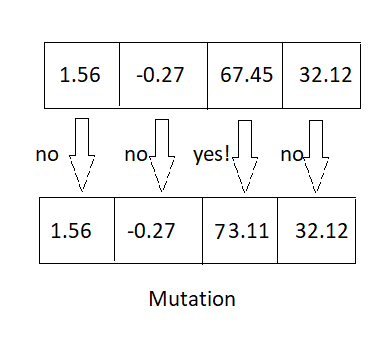
\includegraphics[scale=1]{mutation.png}
	\caption{Mutation process on DNA genotype}
	\label{fig:mutation}
\end{figure}
The process is shown in Figure \ref{fig:mutation}. The behavior of system is greatly affected by mutation rate. Obviously, higher mutation rate say 80\% would nullify the evolutionary process. If major parts of gene are generated randomly, we can't assure that "fit" genes occur with greater frequency. Following algorithm mutate child's genes based on mutation probability.
\begin{lstlisting}[caption=Mutating genes array based on mutation rate]
void mutate(genes, mutation_rate) {
	for (let i = 0; i < 4; i++) {
		if(random(1) < mutation_rate) {
			if(i < 2)  // Attraction/Repulsion
				genes[i] = genes[i] + random(-0.2, 0.2);
			else 	// sensing radius
				genes[i] = genes[i] + random(-10, 10);
		}
	}
}
\end{lstlisting}
\section{Experimental World}
Now we have all pieces in place to validate the above. A two dimensional world of artificial organisms is created and each organism is controlled by network using the described development system. Evolution is governed by natural selection. No universal rule exist to delete organisms; this is under their own control. Each organism has a facing direction which is set randomly at birth. Sharp points indicate their direction. Figure \ref{fig:ecosystem} shows organisms with dominant radius are more fit(green) as compared to the ones with smaller search radius. Putting entire system together in Algorithm 1.
\begin{algorithm}
\caption{Genetic Algorithm: Evolving Ecosystem}
\begin{algorithmic} 
\STATE \textbf{Initialize:} Generate population of N organisms with random DNA.
\LOOP
\FOR{\textit{each alive organism}}                    
\STATE Update organism position vectors.
\STATE Call eatFood and eatPoison procedures.
\STATE Call reproduce procedure for current organism.
\IF{\textit{child is born}}
\STATE Add born child to population.
\ENDIF
\ENDFOR
\ENDLOOP
\end{algorithmic}
\end{algorithm}
%%===========================WORLD===========================
\begin{figure}
	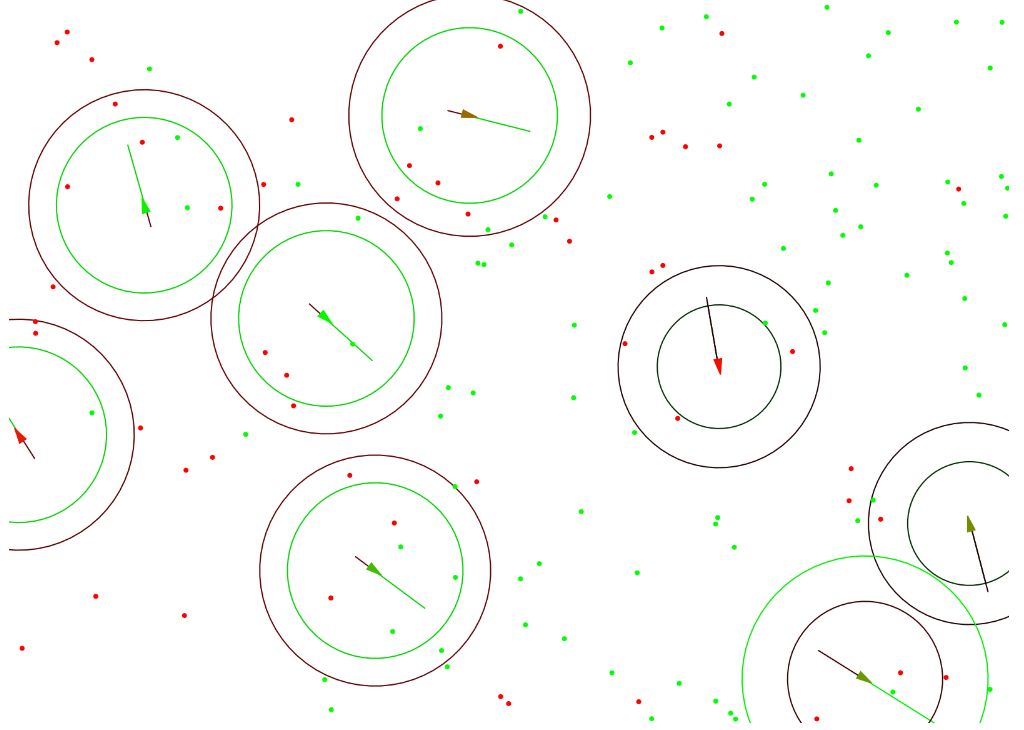
\includegraphics[scale=0.329]{ecosystem.png}
	\caption{Ecosystem Simulation}
	\label{fig:ecosystem}
\end{figure}

\section{Results}
\begin{itemize}
\item \textbf{Convergence and similarity:} When organism reproduce, the child's network almost resembles the parent's network. Examination of experimental world shows resemblance between many of them. Throughout the evolution, population remains converged in small number of species(choosing the reproduction and mutation rate carefully). The fitness criteria also met the developmental landscape, making it appropriate for long-term evolution.
\item \textbf{Increasing Complexity:} For a short period, the organisms with basic genotype move randomly across the system. For next two to three thousand frames(iterations), we find organism's strategy of only eating food(or otherwise die) and having high repulsion to poison. At lateral stages when food is left in small proportion as compared to poison; organisms die but don't eat poison. Some networks do better than others but not so well to display a dominating effect. Success is understandable if we watch it in action.
\end{itemize}
Some organisms with lower food detection radius but higher poison detection radius do well(live longer) because of attraction/repulsion genes. Once the food is in range, high attraction to food steers the organism towards it abruptly(may be previously it was going to eat poison). If there are dominant organisms in ecosystem, then the world always have space for next generation to exist.\\ Taking count of number of organisms born and died, suggest that further generation emerge. However, behavior level analysis is difficult. Observation reveals that current generation share characters with previous species but are still different. Population also start remaining steady after typical run.
%%===========================BIRTH-DEATH===========================
\begin{figure}
	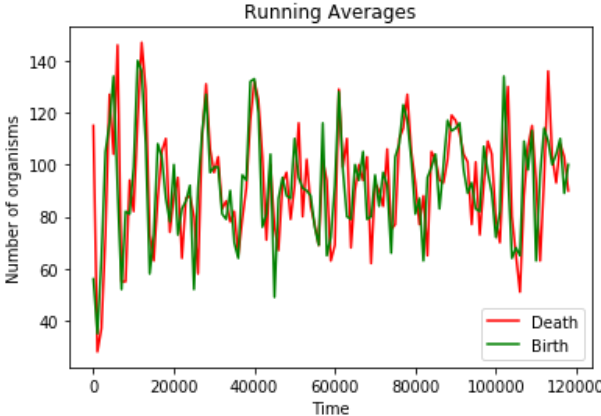
\includegraphics[scale=0.55]{birth-and-death.png}
	\caption{Regular run: organisms birth and death count}
	\label{fig:birth-and-death}
\end{figure}

\section{Conclusion and Future work}
The organisms natural selection in its environment is completely analogous to fitness function based algorithm; hence approach is viable. Selection and reproducing system results in similar looking genotypes and phenotypes with gradual variation over long-term evolution. This also makes clear that certain operations at low-level can obstruct and limit the evolution(birth \& mutation rate). Once an organism has evolved, it can sustain itself for a period of time. We can implement crossover and mutation between two parent organisms when they are in certain proximity of each other. We can make organisms with gender. Can we create a scenario in which organism learn to cooperate with each other; can revive a dying organism.

\begin{thebibliography}{9}
\bibitem{channon&damper} 
Channon, Alastair D., and R. I. Damper. "Evolving novel behaviors via natural selection." (1998): 384-388.
 
\bibitem{Stanley} 
Stanley, Kenneth O., and Risto Miikkulainen. "Evolving neural networks through augmenting topologies." Evolutionary computation 10.2 (2002): 99-127.
 
\bibitem{algorithms-and-experiments} 
Rodzin, Sergey, Olga Rodzina, and Lada Rodzina. "Neuroevolution: problems, algorithms, and experiments." 2016 IEEE 10th International Conference on Application of Information and Communication Technologies (AICT). IEEE, 2016.

\bibitem{feature-selection}
Xue, Bing, et al. "A survey on evolutionary computation approaches to feature selection." IEEE Transactions on Evolutionary Computation 20.4 (2015): 606-626.

\bibitem{evolvable-machines}
Ryerkerk, Matt, et al. "A survey of evolutionary algorithms using metameric representations." Genetic Programming and Evolvable Machines (2019): 1-38.

\bibitem{swarm-evolutionary-computing}
Darwish, Ashraf, Aboul Ella Hassanien, and Swagatam Das. "A survey of swarm and evolutionary computing approaches for deep learning." Artificial Intelligence Review (2019): 1-46.

\bibitem{improving-neuroevolution}
Maul, Tomás H. "Improving Neuroevolution with Complementarity-Based Selection Operators." Neural Processing Letters 44.3 (2016): 887-911.

\bibitem{online-neuroevolution}
Agogino, Adrian, Kenneth Stanley, and Risto Miikkulainen. "Online interactive neuro-evolution." Neural Processing Letters 11.1 (2000): 29-38.

\bibitem{soccer-game-evolution}
Sugisaka, Masanori, Xiaoshu Wang, and Ju-Jang Lee. "Genetic algorithms (GAs) to evolve multiple-agent cooperative systems." Artificial Life and Robotics 3.3 (1999): 139-142.

\bibitem{mapping-genotype-phenotype}
Ekárt, Anikó, and Peter R. Lewis. "Genotype–phenotype mapping implications for genetic programming representation: Commentary on “On the mapping of genotype to phenotype in evolutionary algorithms” by Peter A. Whigham, Grant Dick, and James Maclaurin." Genetic Programming and Evolvable Machines 18.3 (2017): 369-372.

\bibitem{array-selection}
Mohamad, Mohd Saberi, et al. "Gene subset selection using an iterative approach based on genetic algorithms." Artificial Life and Robotics 14.1 (2009): 12-15.

\bibitem{GA-and-machine-learning}
Goldberg, David E., and John H. Holland. "Genetic algorithms and machine learning." Machine learning 3.2 (1988): 95-99.


\end{thebibliography}
\end{document}